\section{语法分析——自上而下}
\subsection{语法分析器的功能}

语法分析是编译过程的核心部分。它的任务是在词法分析识别出单词符号串的基础上,分析并判定程序的语法结构是否符合语法规则。

\begin{figure}[H]
    \centering
    \begin{tikzpicture}[thick,font=\small,inner xsep=1em,inner ysep=1ex]
        \node[draw] (1) at (0,0) {词法分析器}; 
        \node[draw] (2) at (5,0) {语法分析器}; 
        \node[draw,text width=4em] (3) at (10,0) {编译程序后续部分}; 
        \node[draw] (4) at (5,-2) {符号表}; 
        \begin{scope}[-Stealth]
            \draw (-3,0) -> (1) node[pos=0.5,above] {源程序};
            \draw (1.east) ++ (0,0.1) -> ++ (2.3,0) node[pos=0.5,above] {单词符号};
            \draw (2.west) ++ (0,-0.1) -> ++ (-2.3,0) node [pos=0.5,below,font=\footnotesize] {取下一单词符号};
            \draw[dashed] (2) -- (3) node [pos=0.5,above] {语法分析树};
            \draw[dashed] (3) -- ++(3,0);
            \draw[Stealth-Stealth] (1.south) -- (4.west);
            \draw[Stealth-Stealth] (2.south) -- (4.north);
            \draw[Stealth-Stealth] (3.south) -- (4.east);
        \end{scope}
    \end{tikzpicture}
    \caption{语法分析器在编译程序中的地位}
    \label{fig:语法分析器在编译程序中的地位}
\end{figure}

语法分析器的工作本质上就是按文法的产生式,识别输入符号串是否为一个句子。这里的输入串指单词符号(文法的终结符)组成的有限序列。

对一个文法,给出一串(终结)符号时,如何判断它是不是该文法的一个句子?此时要判断能否从文法的开始符号出发推导出这个输入串。或者从概念上,就是要建立一棵与输入串相匹配的语法分析树。

按照语法分析树的建立方法,可以将语法分析办法分成两类,即自上而下分析发法和自下而上分析法。

\subsection{自上而下分析面临的问题}

自上而下语法分析,顾名思义,就是从文法的开始符号出发,向下推导,推出句子。自上而下推导的主旨是:对任何输入串,试图用一切可能的办法,从文法开始符号(根结)出发,自上而下地为输入串建立一棵语法树。或者说,为输入串寻找一个最左推导。

下面举一个简单的例子\footnote{参考书 P67-68,这里为本人理解,叙述为白话,更准确但难懂的形式化语言建议参考原书},假定有文法:
\begin{enumerate}
    \item[(1)] S $\rightarrow$ xAy
    \item[(2)] A $\rightarrow$ **|*
\end{enumerate}

以及输入串$\alpha$: x*y,下面构造 $\alpha$ 的语法树。 

\begin{enumerate}
    \item 首先按文法开始符号产生根结 P,并让指示器 IP 指向输入串的第一个符号 x。然后用 S 的规则(此处只有一条)绘制树。
    \begin{figure}[H]
        \centering
        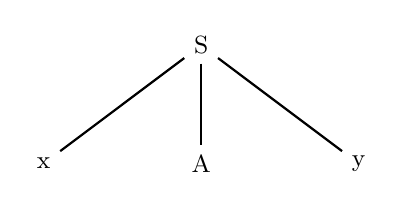
\begin{tikzpicture}[font=\small]
            \node (S) at (0,0) {S};
            \node (x) at (-2,-1.5) {x};
            \node (A) at (0,-1.5) {A};
            \node (y) at (2,-1.5) {y};
            \draw[thick] (S) -- (x);
            \draw[thick] (S) -- (A);
            \draw[thick] (S) -- (y);
        \end{tikzpicture}
    \end{figure}
\end{enumerate}



























\newpage